%!TEX root = ../../thesis.tex
\define{\chapterpath}{\allchapterspath/bci}
\define{\imgpath}{\chapterpath/img}

\chapter{Application to Brain Computer Interaction}
\label{chapter:bci}
\minitoc

With I\~naki Iturrate and Luis Montesano.

Context - Why now: We have a working algorithm, in simulation or with pretty god data

Need - Why the reader: we want to test it on a realistic setup with signal which make sense to use in tis context, BCI seems a promising direction

Task - Why us: Together with I\~naki Iturrate and Luis Montesano we adapted the algorithm to work with EEG signal on a grid world setup.

Object- Why this chapter:  We present first the EEG paradigm and related work in the domain. Then show simulated experiment using prerecorded data, and finally show some run with some real users.

Findings - What: It works online, with naive subject, and without pre-calibration, but the performance are no the same than in simulation

Conclusions - So what: We can hope to release this algorithm in the real word and make it useful to use. EEG are among the hardest signal to classify, if we can do it with them, we sure can do it with other king of signals.

Perspectives - What now: That are only toy problem, discrete state, discrete action, where should we go next? What are the current limitation?

Recent works have explored the use of brain signals to directly control virtual and robotic agents in sequential tasks. So far in such brain-computer interfaces (BCIs), an explicit calibration phase was required to build a decoder that translates raw EEG signals from the brain of each user into meaningful feedback signals.
%
This paper proposes a method that removes the need for such a calibration phase, and allows a user to control an agent to solve a sequential task.
%
The proposed method assumes a distribution of possible tasks, and infers the interpretation of EEG signals and the task by selecting the hypothesis which best explains the history of interaction. 
%
Also, we use a measure of uncertainty of the task and of the EEG signal interpretation as an exploratory reward for a planning strategy, and this speeds up learning by guiding the system to regions that help disambiguate among task hypotheses.
%
We report experiments where four users control, by means of a BCI, an agent on a virtual world to reach a target without any previous calibration process.

%%%%%%%%%%%%%%%%%%%%%%%%%%%%%%%%%%%%%%%%%%%%%%
%%%%%%%%%%%%%%%%%%%%%%%%%%%%%%%%%%%%%%%%%%%%%%
%%%%%%%%%%%%%%%%%%%%%%%%%%%%%%%%%%%%%%%%%%%%%%
%%%%%%%%%%%%%%%%%%%%%%%%%%%%%%%%%%%%%%%%%%%%%%
%%%%%%%%%%%%%%%%%%%%%%%%%%%%%%%%%%%%%%%%%%%%%%
\section{BCI control using Error Related Potential}

evaluation scenarios were tested with two different types of signals: artificial datasets, and real ErrP datasets recorded from previous experiments \cite{iturrate2013task}.

\paragraph{EEG datasets}
Once the algorithm was evaluated with artificial datasets, we tested the feasibility of the proposed self-calibration approach using real ErrP datasets. The objective of this analysis is to study the scalability of our method to EEG data, which may have different properties than our artificial dataset. 

The EEG data were recorded in a previous study \cite{iturrate2013task} where participants monitored on a screen the execution of a task where a virtual device had to reach a given goal. The motion of the device could be correct (towards the goal) or erroneous (away from the goal). The subjects were asked to mentally assess the device movements as erroneous or non-erroneous. The EEG signals were recorded with a gTec system with 32 electrodes distributed according to an extended 10/20 international system with the ground on FPz and the reference on the left earlobe. The ErrP features were extracted from two fronto-central channels (FCz and Cz) within a time window of $[200,700]$ ms (being 0 ms the action onset of the agent) and downsampled to $32$ Hz. This leaded to a vector of $34$ features.

\paragraph{Comparison with calibration methods}
In order to show the benefit of learning without explicit calibration, we compare our method with the standard supervised BCI calibration procedure. In this calibration procedure, which can last for up to 40 minutes, the experimenter needs to record enough data from the user from several offline runs, where the user is not controlling the agent but just passively assessing its actions.
%
Following the literature on ErrPs \cite{chavarriaga2010learning,iturrate2013task} our training data will consist of 80 percent of positive examples (associated to a correct feedback) and 20 percent of negative examples (associated to an incorrect feedback). Our proposed algorithm is compared with different (but standard) sizes of calibration datasets: 200, 300 and 400 examples.




\subsection{EEG datasets and comparison with calibration method}

\paragraph{Example}
Figure~\ref{fig:sequence} shows one particular run of 500 steps comparing our self-calibration method with a calibration procedure of 400 steps. The two independent runs use as real EEG dataset with $80\%$ ten-fold classification accuracy. As our algorithm is operational from the first step, it can estimate the real task when sufficient evidence has been collected. On the other hand, a calibration approach collects signal-label pairs for a fixed number of steps and use the resulting classifier without updating it. This provokes that, during the calibration phase, no tasks can be learned, substantially delaying the user's online operation.

\begin{figure}[!ht]
\centering
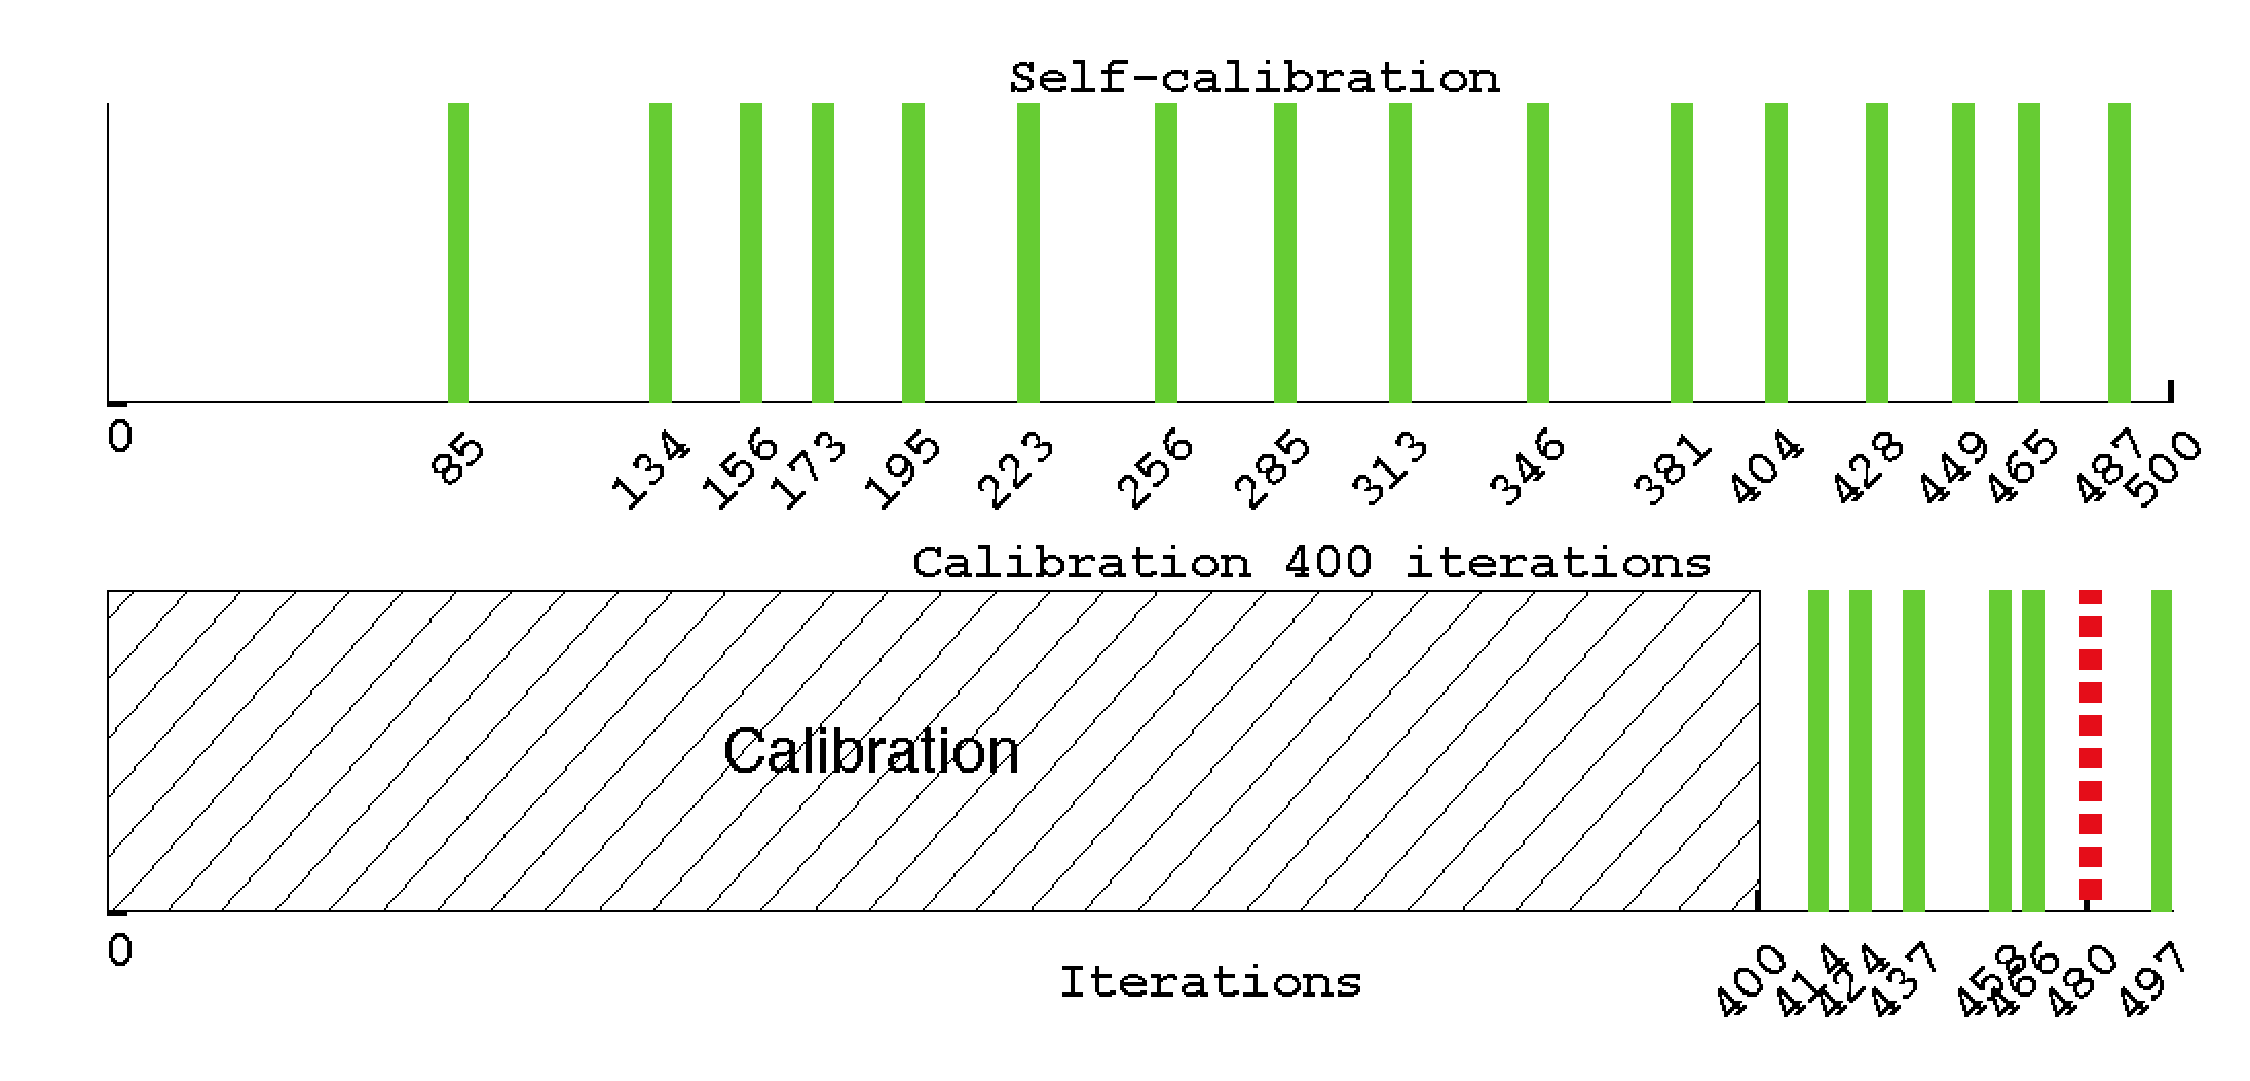
\includegraphics[width=\plotsize\columnwidth]{\imgpath/plot_the_aaai_sequence.eps}
\caption{Time-line of one run from EEG dataset of $80$ percent ten-fold classification accuracy, self-calibration (top) versus 400 steps calibration (bottom). Green (filled) and red (dashed) bars represents respectively correct and incorrect task achievement. The proposed self-calibration method allow to reach a first task faster than would take a calibration procedure.}
\label{fig:sequence}
\end{figure} 



Figure~\ref{fig:sequence_evolution} shows the evolution of classification rate between our self-calibration method with a calibration procedure of 400 steps. As our method assigns different labels to each new teaching signal, the resulting classifiers have different performances, which help identifying the correct task. Once a task is identified (e.g.\ step 85 and 134), the corresponding labels are taken as ground truth, and all classifiers will have the same accuracies. As the agent starts exploring again to estimate the new tasks, all the classifiers except the true one will start to have worse accuracies again.

\begin{figure}[!ht]
\centering
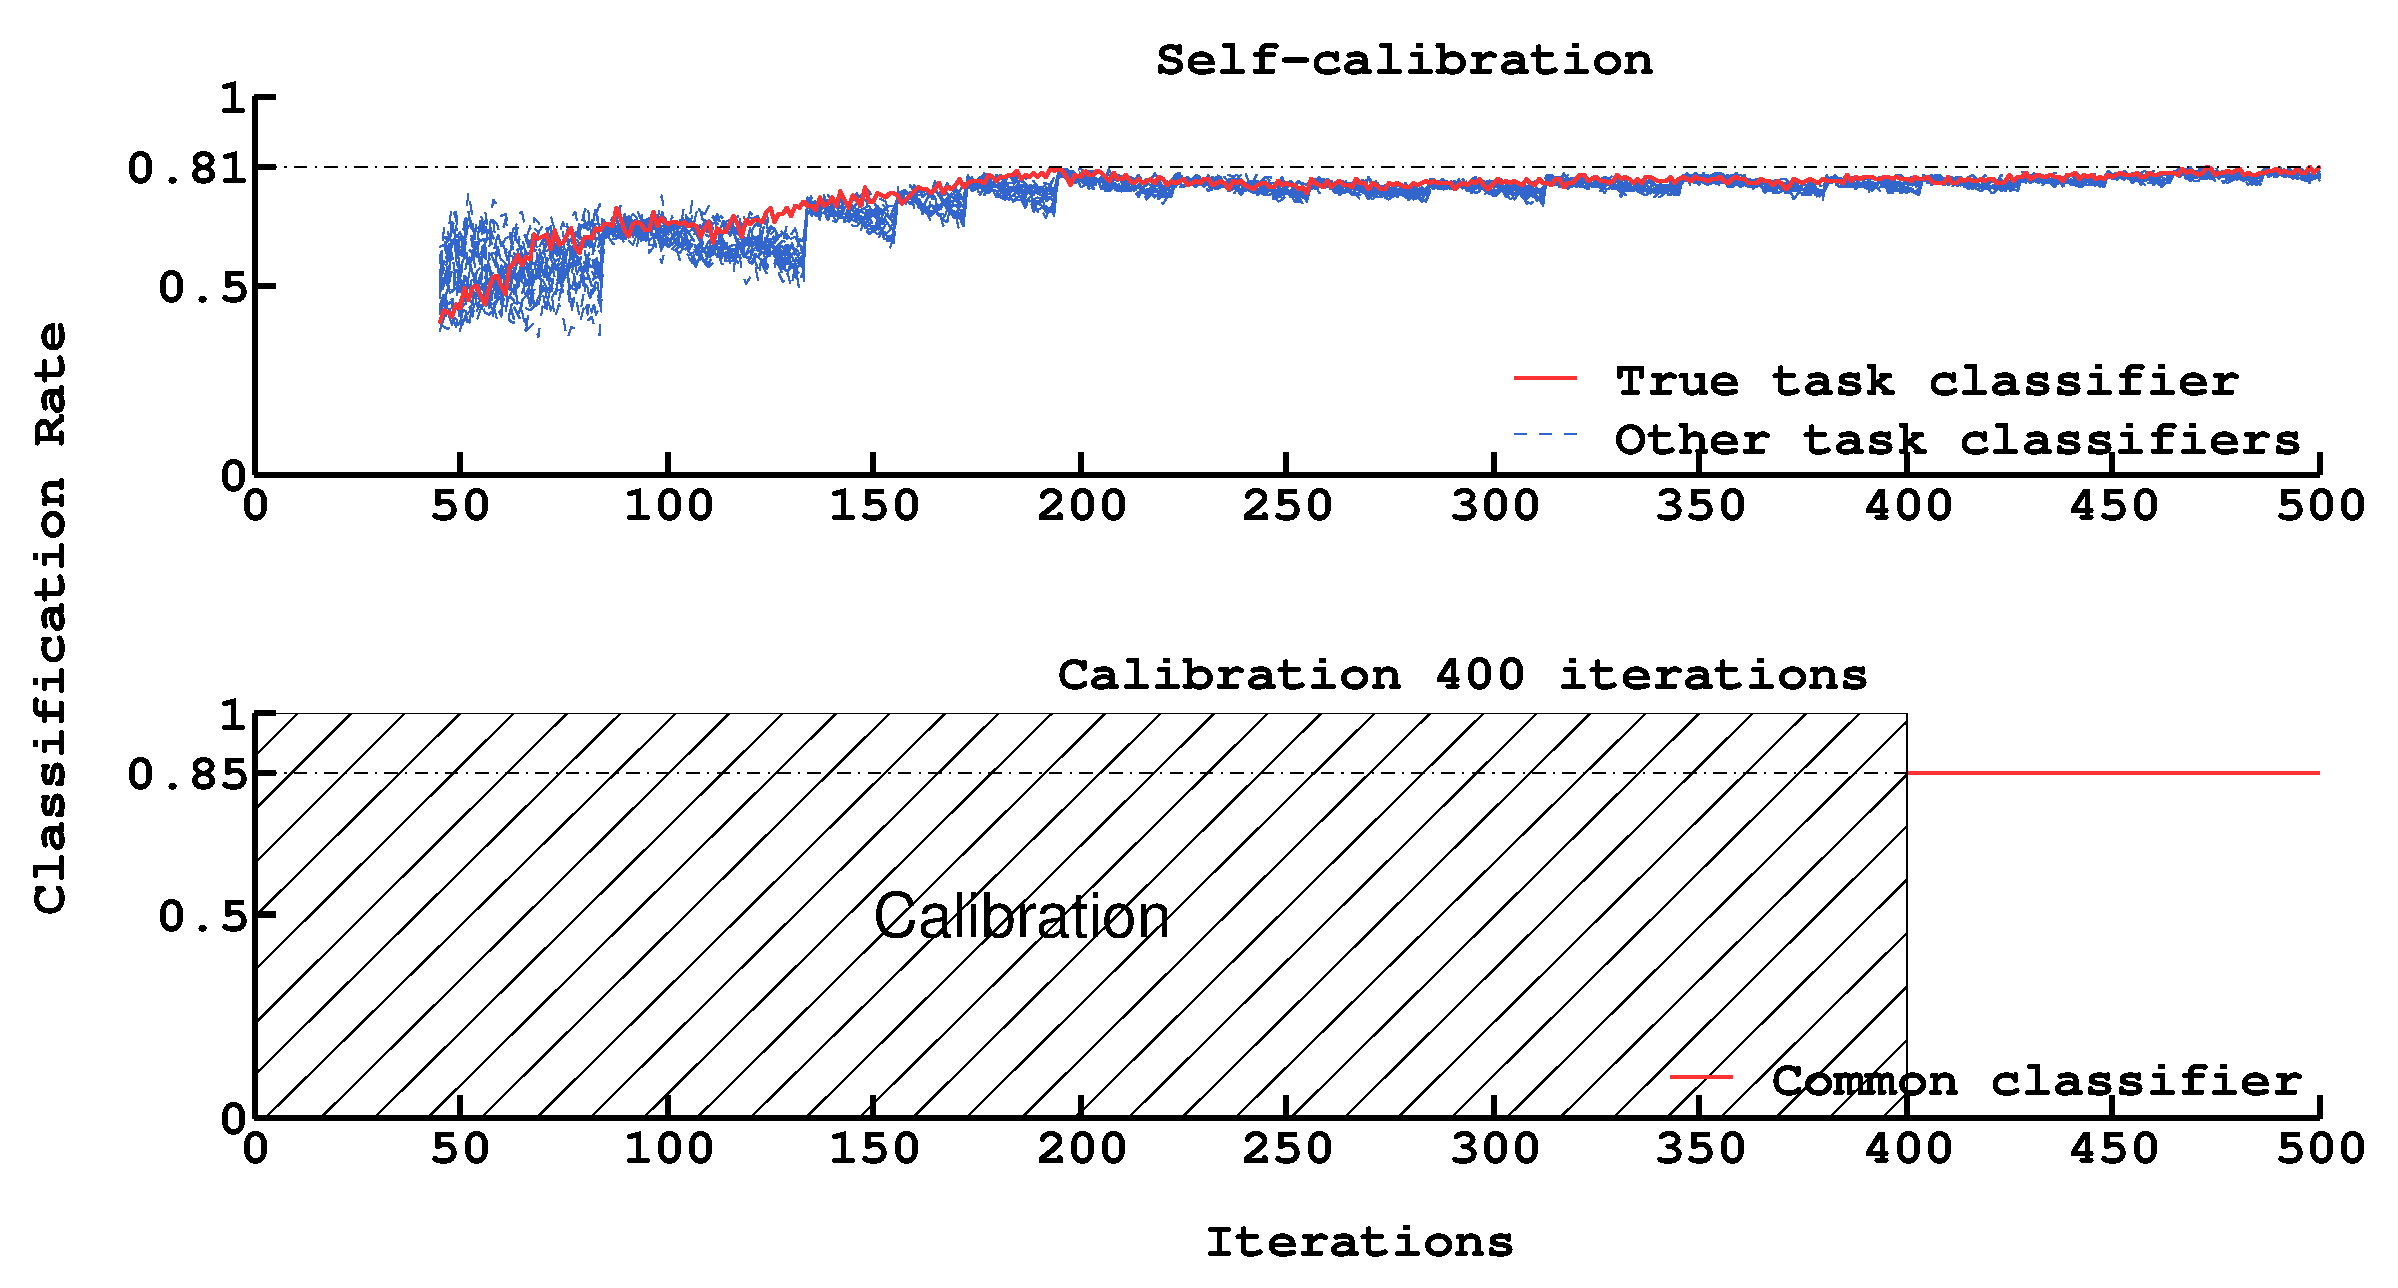
\includegraphics[width=\plotsize\columnwidth]{\imgpath/plot_evo_classification_rate.eps}
\caption{Evolution of classification rate of one run from EEG data, self-calibration (top) versus 400 steps calibration (bottom). On top, the red line represents the classifier corresponding to the successive tasks taught by the user, the dashed blue lines represent all others tasks. Our method updates classifiers every steps.}
\label{fig:sequence_evolution}
\end{figure} 

\paragraph{Time to first task}

Figure~\ref{fig:firstEEG} shows the results per group of dataset. Our algorithm allows to complete the first task without errors and in a fair amount of iteration.  For our method, the learning time is strongly correlated with the dataset quality. However calibration methods, which do not update their classifier once calibrated, identify more tasks incorrectly.

\begin{figure}[!ht]
\centering
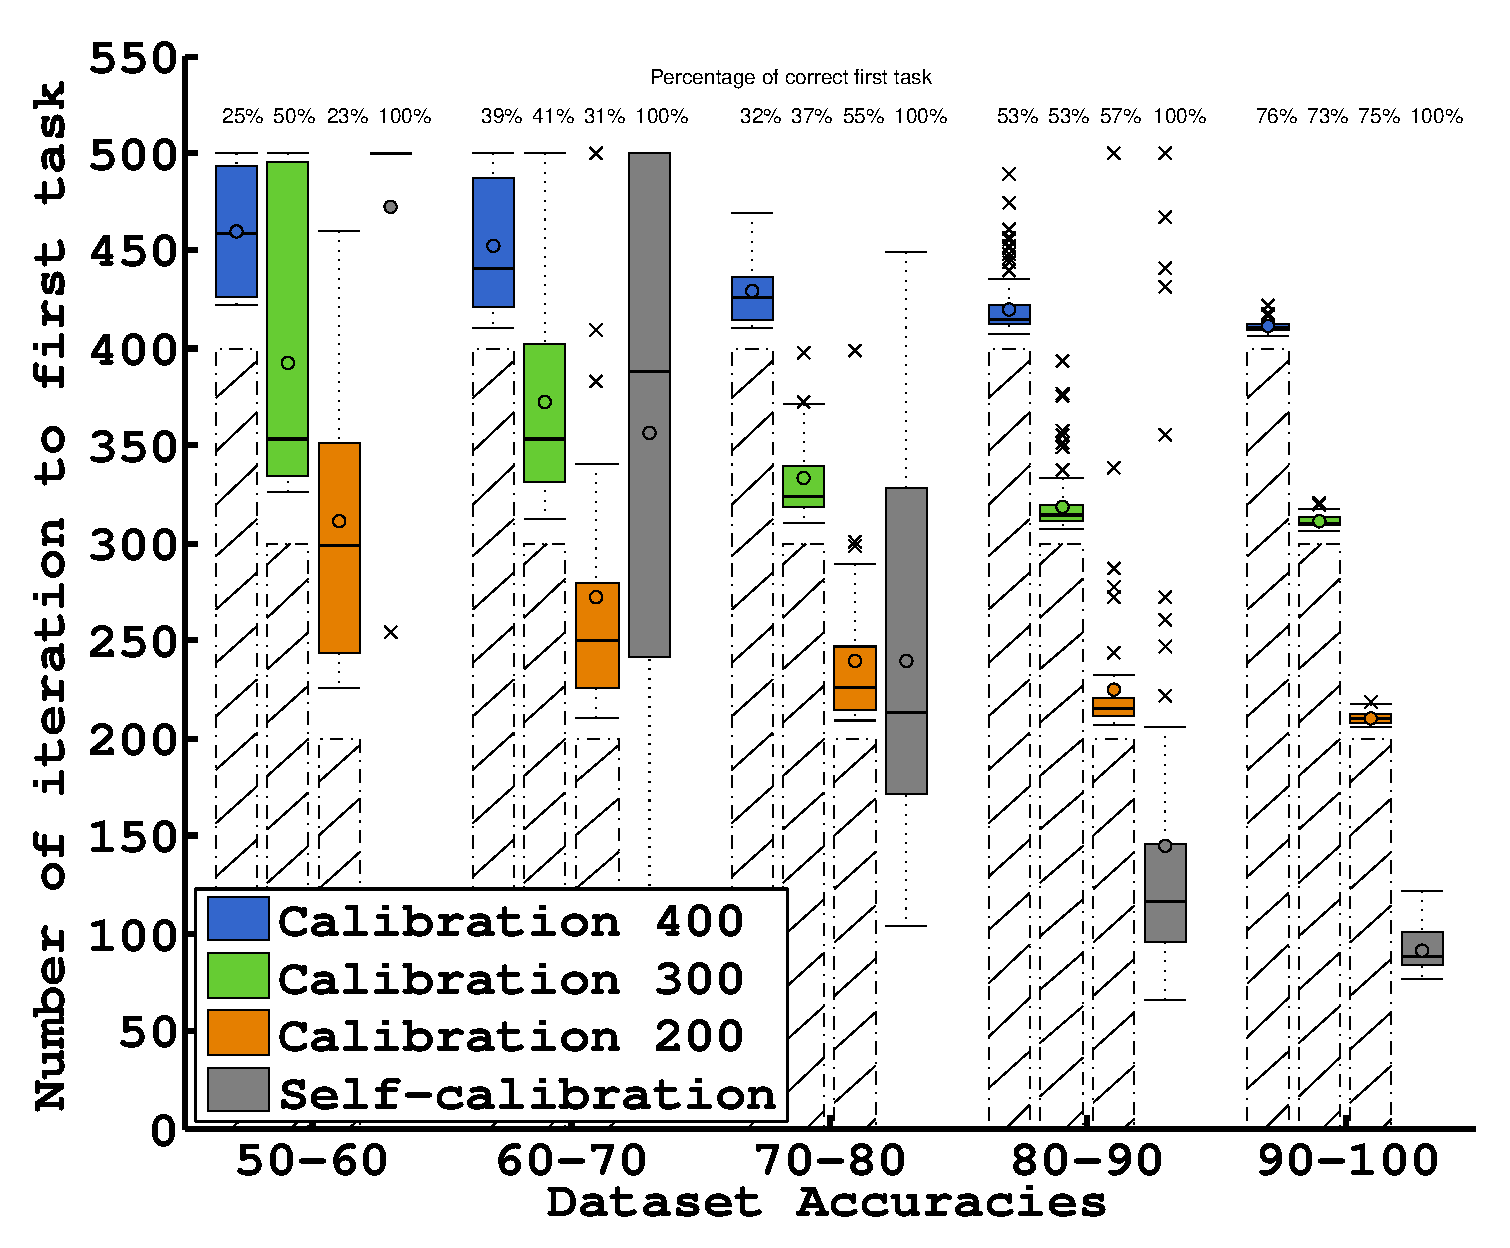
\includegraphics[width=\plotsize\columnwidth]{\imgpath/plot_EEG_calib_firstconf.eps}
\caption{Number of steps to complete first task with EEG data. The method scale well to EEG data. Contrary to the standard calibration approaches, we do not make mistakes with low quality datasets.}
\label{fig:firstEEG}
\end{figure} 

%We can identify two main differences between our method and the usual calibration procedure for this kind of BCI experiments:
%\begin{enumerate}
%\item \textbf{Positive/Negative percent ratio of training examples}. Following the literature \cite{chavarriaga2010learning, iturrate2013task} we used a 80/20 percent ratio. Table \ref{tab:correctLabelRatio} shows the positive/negative ratio obtained following our planning method. The ratio we obtain is more balanced, resulting in classifiers with better properties. However a 50/50 percent ratio may lead to practical problems during online real world experiments and should be studied in more details, see open questions in section \ref{sec:conclusion}.
%\item \textbf{Online update of multiple classifiers.} Our method integrates new data at every step whose label can differ between task hypothesis. For incorrect task hypothesis, the associated label can be incorrect and decrease the performance of the associated classifier, see figure \ref{fig:planningExplained}c. This dynamic can be observed in figure \ref{fig:sequence_evolution} where classifiers associated to incorrect tasks (in blue) have lower estimated accuracies than the correct one (in red). As a result our algorithm makes different predictions and updates for each hypothesis.
%\end{enumerate}

%\begin{table}
%\begin{tabular}{c c c}
%Dataset Accuracies & Self-calibration & Calibration \\ \hline
%50-60 & 0.48 (0.02) & 0.8 (0) \\
%60-70 & 0.50 (0.03) & 0.8 (0) \\
%70-80 & 0.53 (0.03) & 0.8 (0) \\
%80-90 & 0.57 (0.03) & 0.8 (0) \\
%90-100 & 0.59 (0.01) & 0.8 (0) \\
%\end{tabular}
%\caption{Mean ratio of positive examples in training dataset (standard deviation shown in parenthesis). Calibration procedure for ErP EEG signal usual account for a 80 percent ratio of positive examples. However when following our method we collect as many positive than negative examples, see discussion in section \ref{sec:conclusion}.}
%\label{tab:correctLabelRatio}
%\end{table}

%\begin{figure}[!ht]
%\centering
%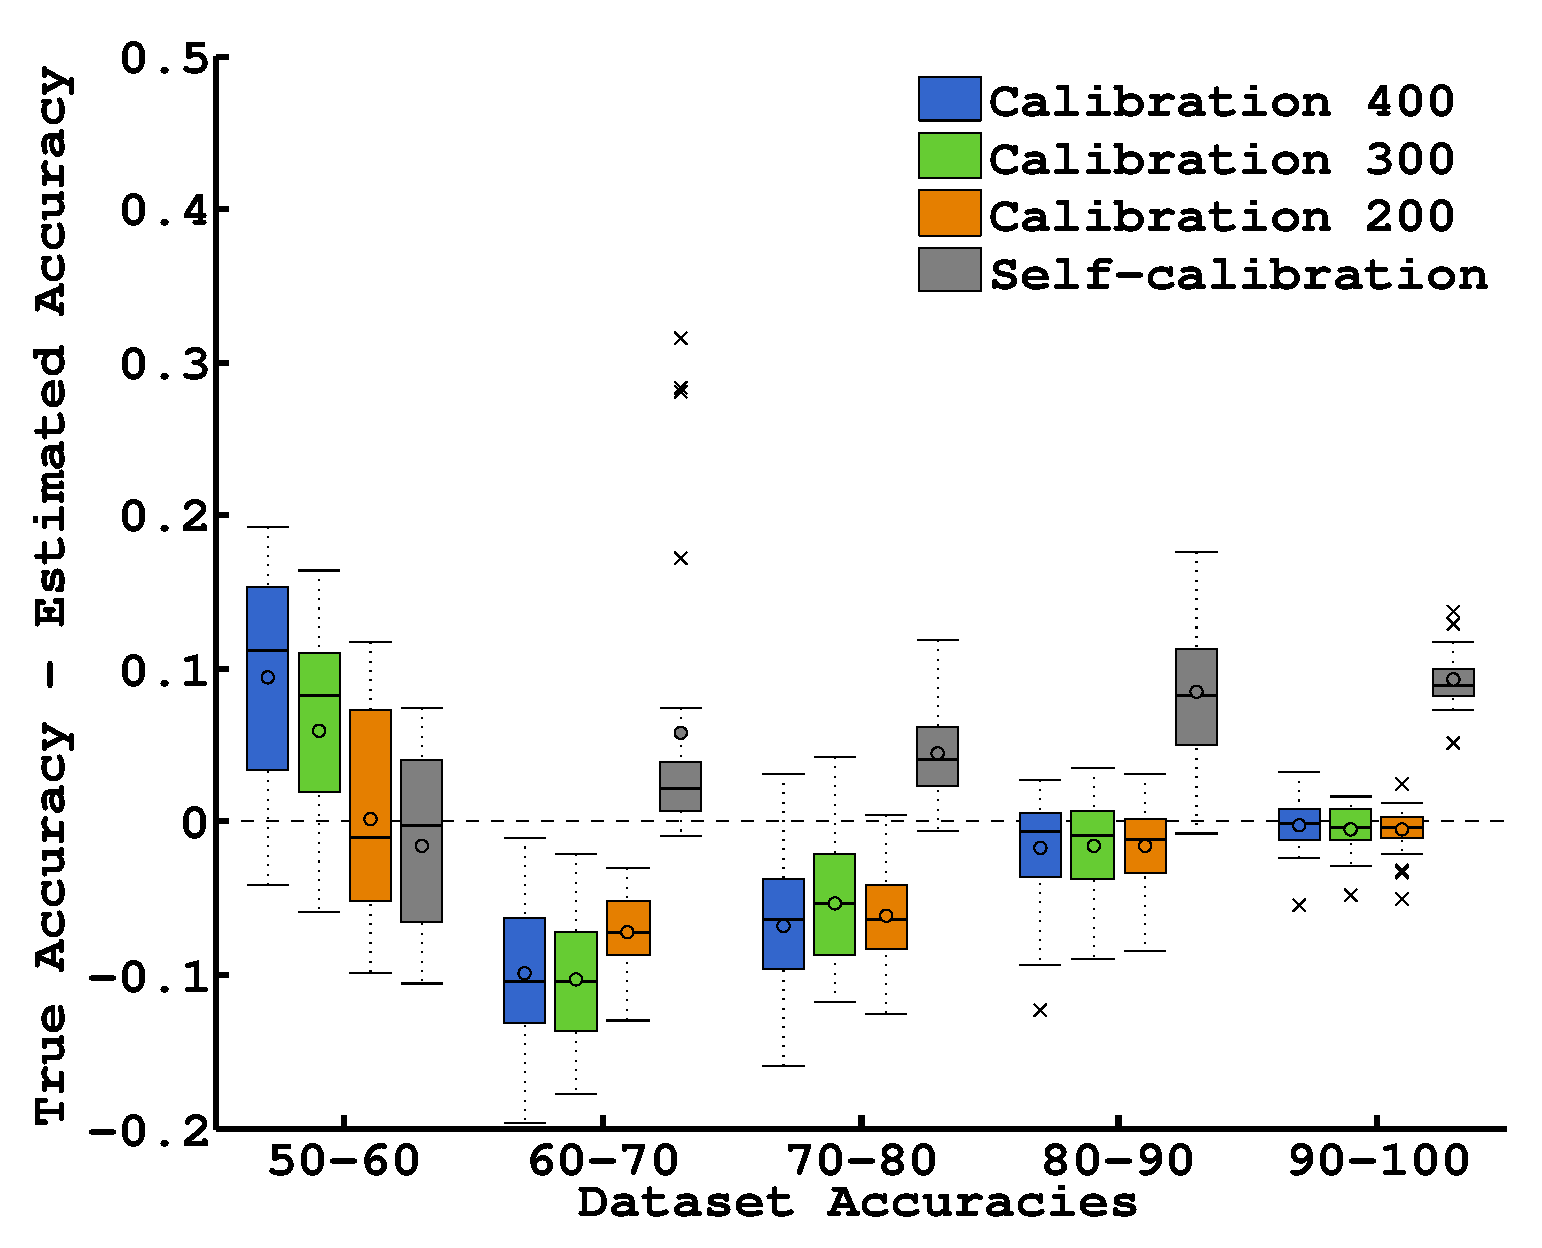
\includegraphics[width=\plotsize\columnwidth]{\imgpath/plot_explaination_for_calib_failure.eps}
%\caption{Difference between true accuracy and estimated accuracy. True accuracy is the performance of the classifier on the unused data. Estimated accuracy is the 10 fold cross validation performance of the classifier on collected data. A negative(positive) value indicates the classifier is over(under)-estimating its performance. Calibration methods tend to produce over-confident classifiers, certainly due to the biased positive to negative training example ratio, see table \ref{tab:correctLabelRatio}.}
%\label{fig:calibFail}
%\end{figure}

\paragraph{Cumulative performances}

Figure~\ref{fig:nCorrectEEG} compares the number of tasks that can be achieved in 500 steps. With 90\% and more dataset quality we can achieve about 20 tasks on average. The results are consistent with artificial dataset analysis.

\begin{figure}[!ht]
\centering
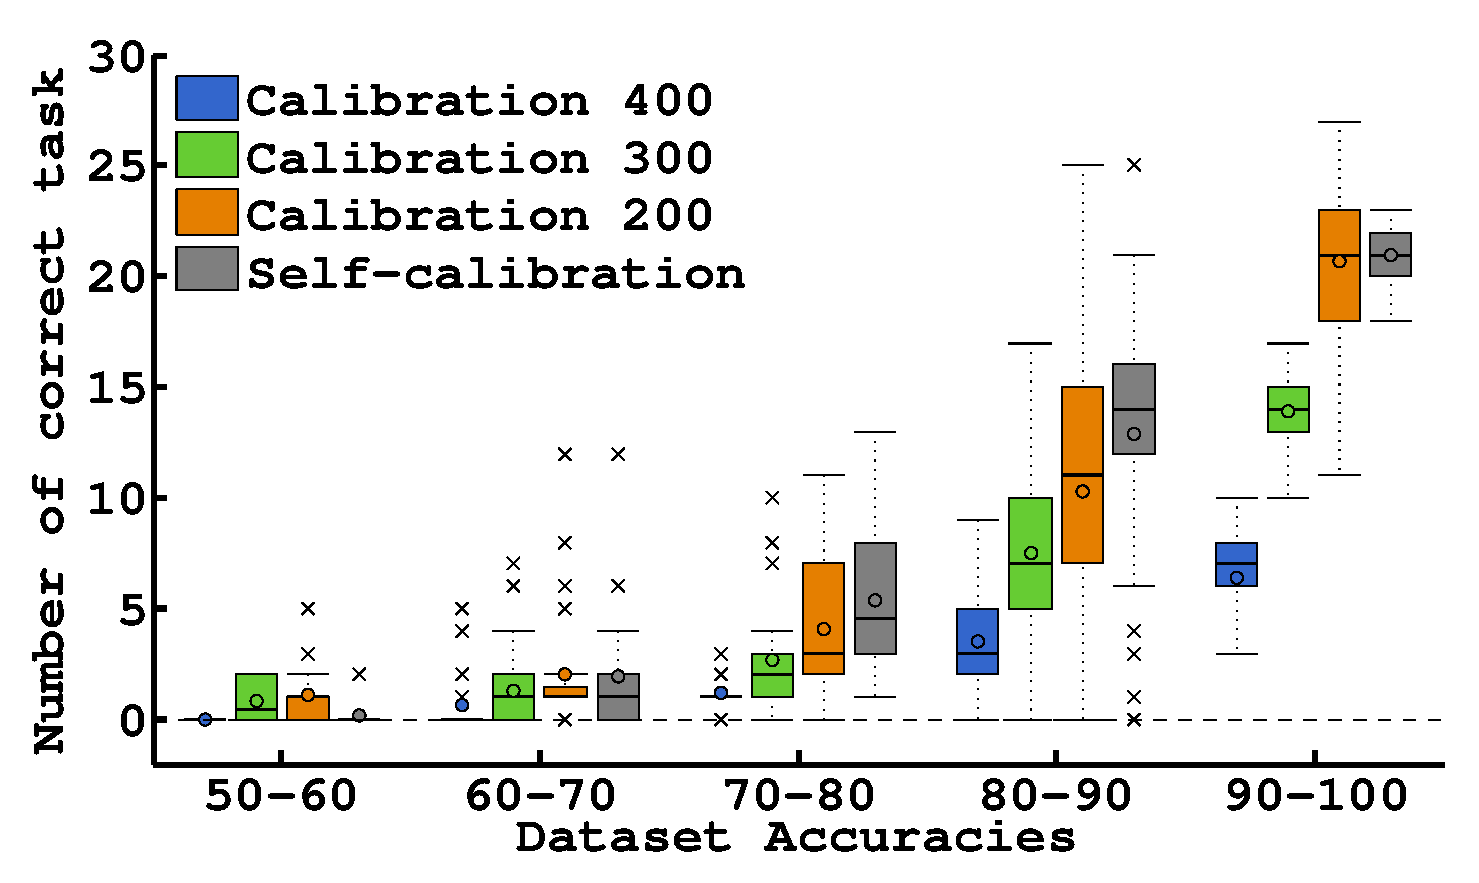
\includegraphics[width=\plotsize\columnwidth]{\imgpath/plot_EEG_calib_nCorrect.eps}
\caption{Number of task correctly achieved in 500 steps with EEG data. Calibration methods can not complete a significant number of task as most of the time is spent on calibration.}
\label{fig:nCorrectEEG}
\end{figure} 

The calibration methods can not complete many task as a significant amount of iteration was used for calibrating the system. A calibration of 200 steps makes as many good estimation than our method, but it also makes many wrong estimation, see Figure~\ref{fig:nWrongEEG}. For calibration methods, the less time spent on calibration, the poorer the classifier which implies more mistakes.

\begin{figure}[!ht]
\centering
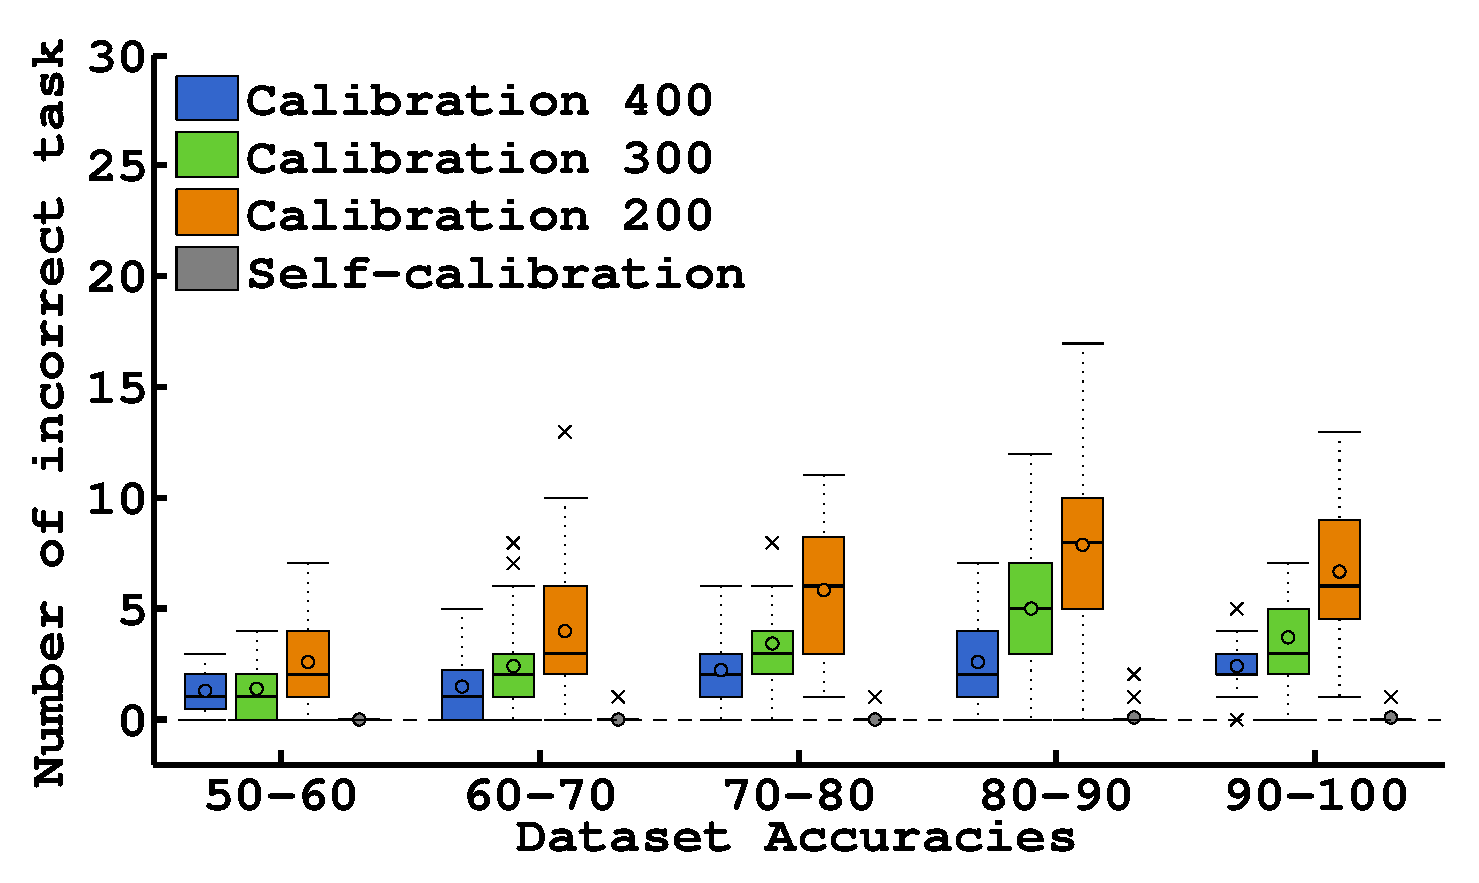
\includegraphics[width=\plotsize\columnwidth]{\imgpath/plot_EEG_calib_nWrong.eps}
\caption{Number of task incorrectly achieved in 500 steps with EEG data. Calibration methods, which do not update their models once calibrated, make more errors.}
\label{fig:nWrongEEG}
\end{figure}

%\paragraph{Last 100 iterations performances}
%
%Figure~\ref{fig:nCorrectEEG_last100} compares the number of task that can be achieved during the last 100 steps with EEG data. With 80-90\% dataset quality, all methods achieve an average success rate of one task every 20 steps. However calibration methods, which do not update their models once calibrated, make more mistakes (see figure \ref{fig:nWrongEEG_last100}).
%
%\begin{figure}[!ht]
%\centering
%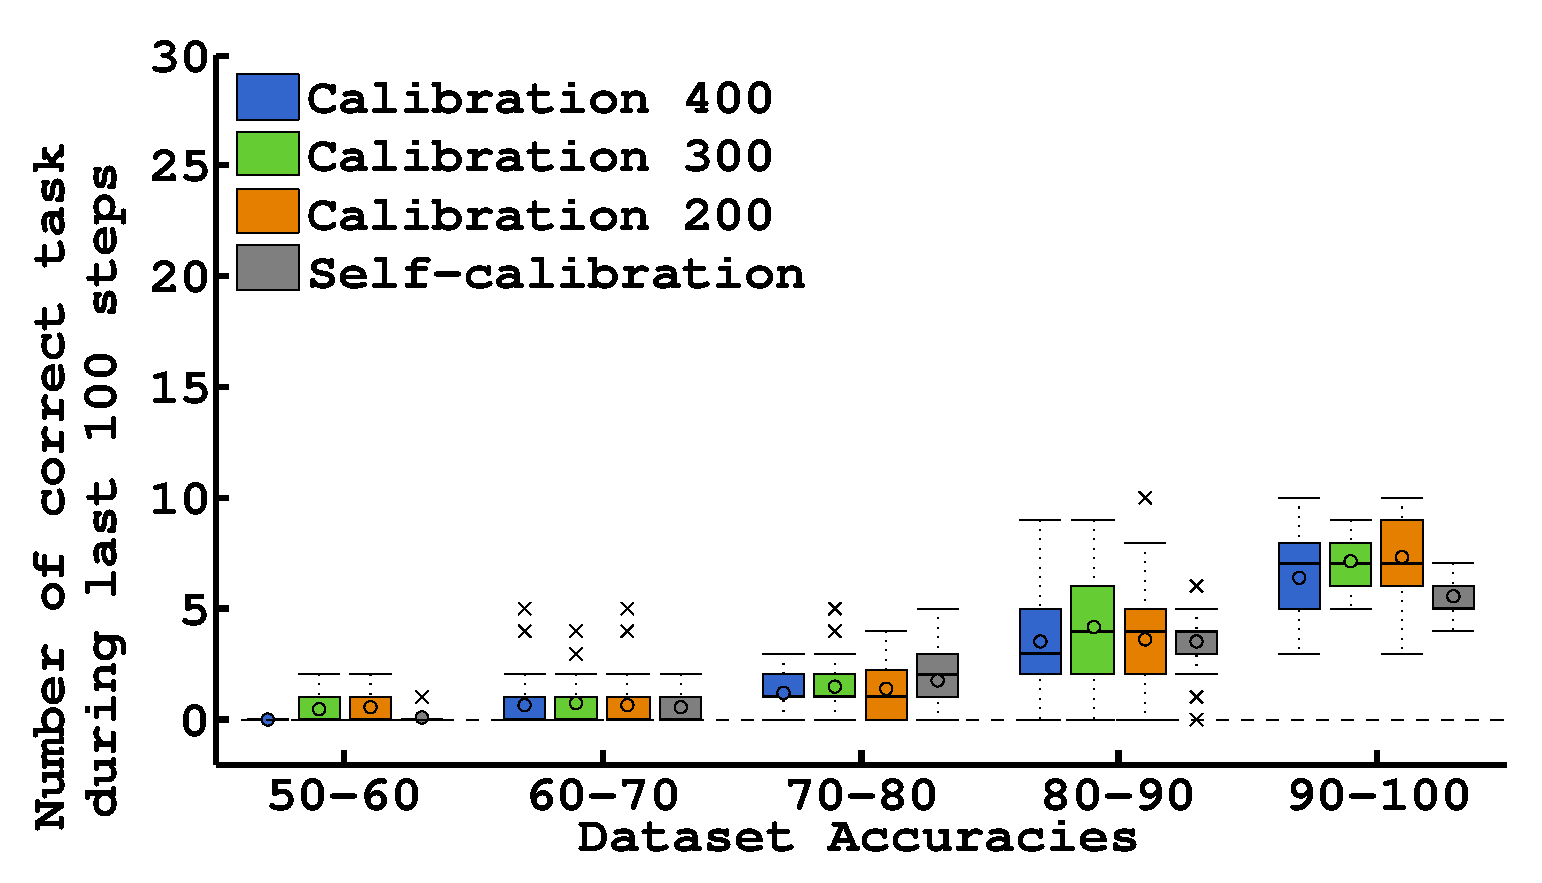
\includegraphics[width=\plotsize\columnwidth]{\imgpath/plot_EEG_calib_nCorrect_last100.eps}
%\caption{Number of task correctly achieved during the last 100 steps with EEG data. All methods have equivalent successful reaching rate.}
%\label{fig:nCorrectEEG_last100}
%\end{figure} 
%
%\begin{figure}[!ht]
%\centering
%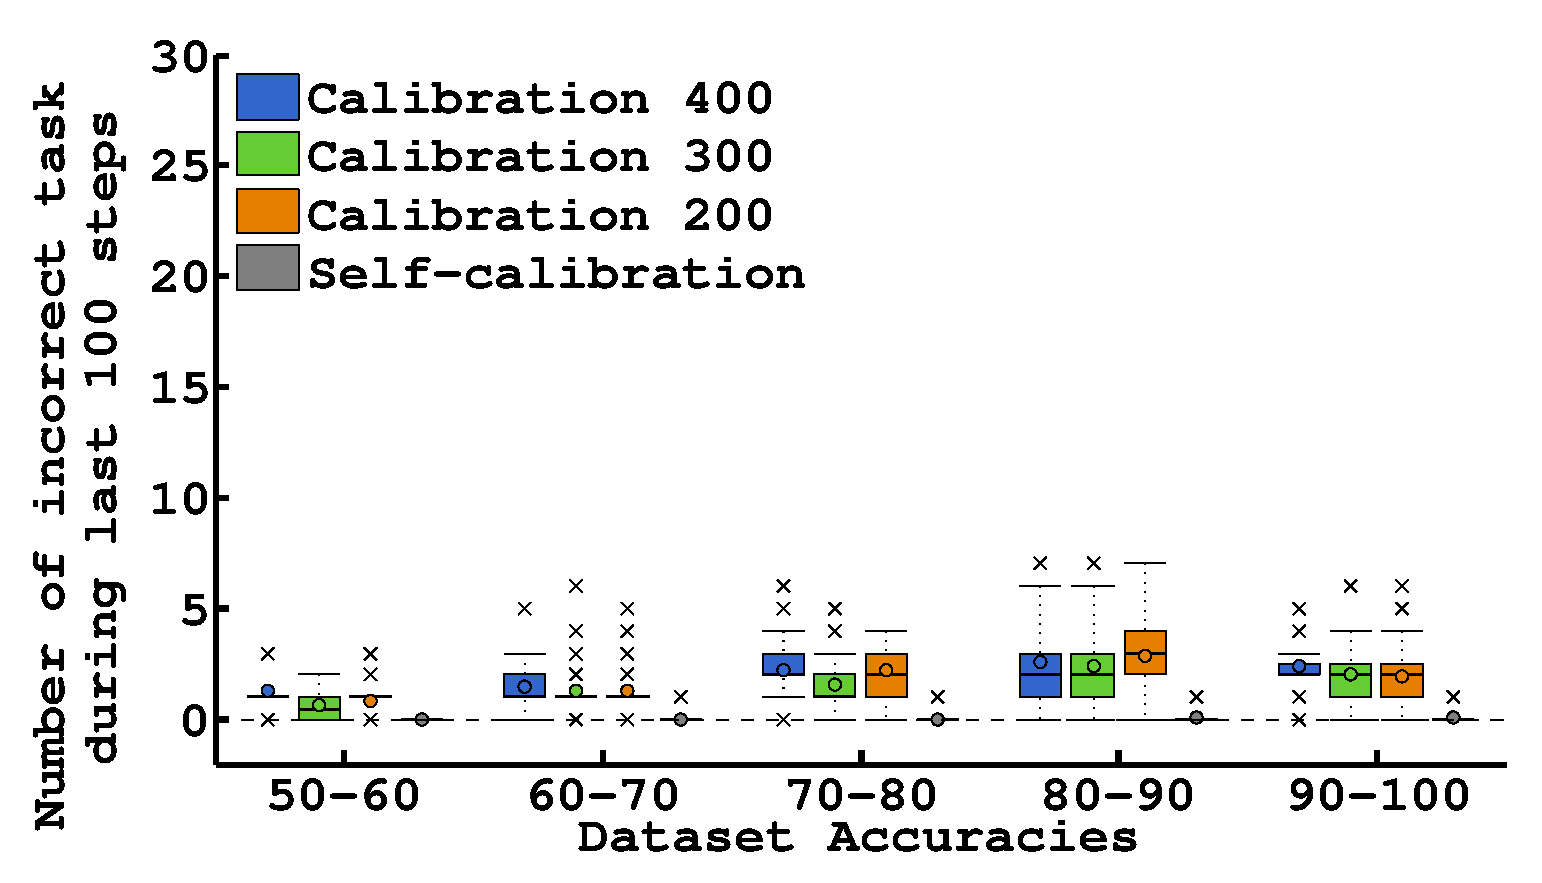
\includegraphics[width=\plotsize\columnwidth]{\imgpath/plot_EEG_calib_nWrong_last100.eps}
%\caption{Number of task incorrectly achieved during the last 100 steps with EEG data. Calibration methods, which do not update their models once calibrated, make more errors.}
%\label{fig:nWrongEEG_last100}
%\end{figure} 

 % shows the number of tasks identified with respect to the accuracy of the dataset, and the number of tasks incorrectly identified. Notice how the number of identified task is correlated to the quality of the dataset. Importantly, we were able to identify 15 to 20 tasks in 500 steps on good quality dataset without the need for a calibration procedure.


% \begin{figure*}[t]
% \centering
% \begin{minipage}[t]{.65\columnwidth}
%   \centering
%       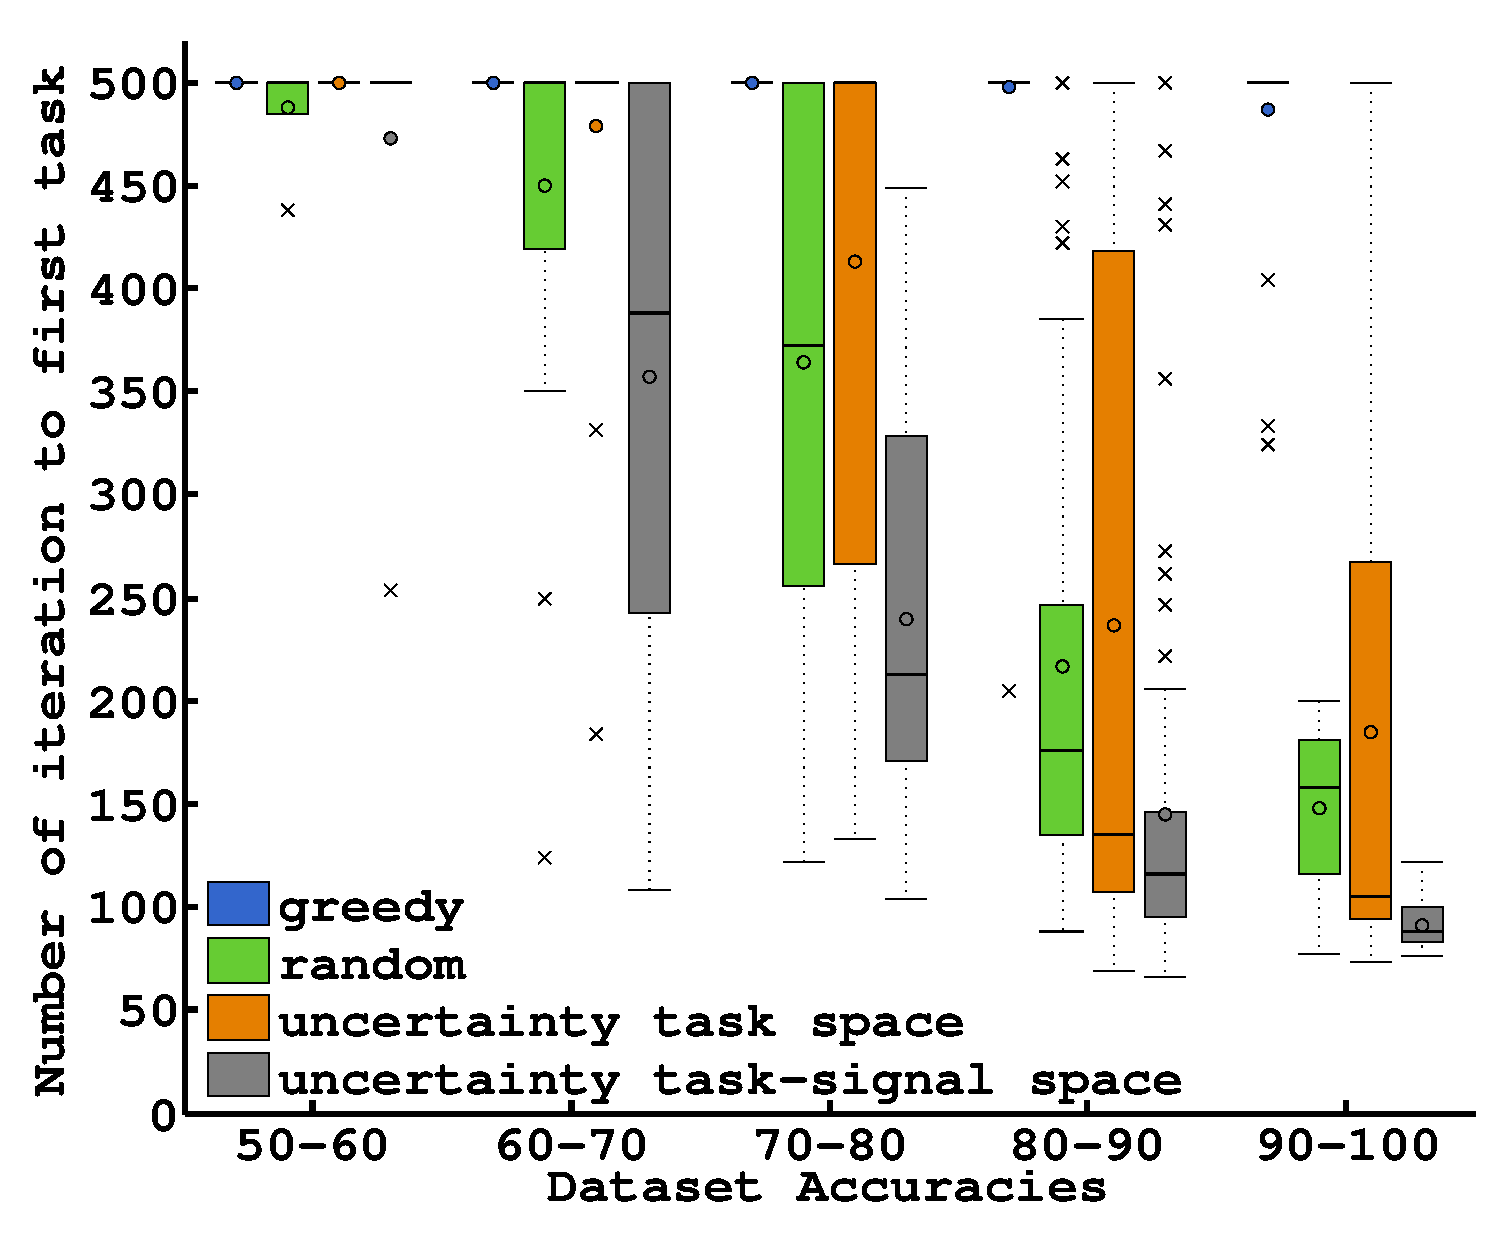
\includegraphics[width=\plotsize\columnwidth]{\imgpath/plot_EEG_planning.eps}
%       \caption{\todo{this is the plot for EEG data, xp are running for artificial data}}
%     \label{fig:planning}
% \end{minipage}
% \begin{minipage}[t]{.65\columnwidth}
%   \centering
%       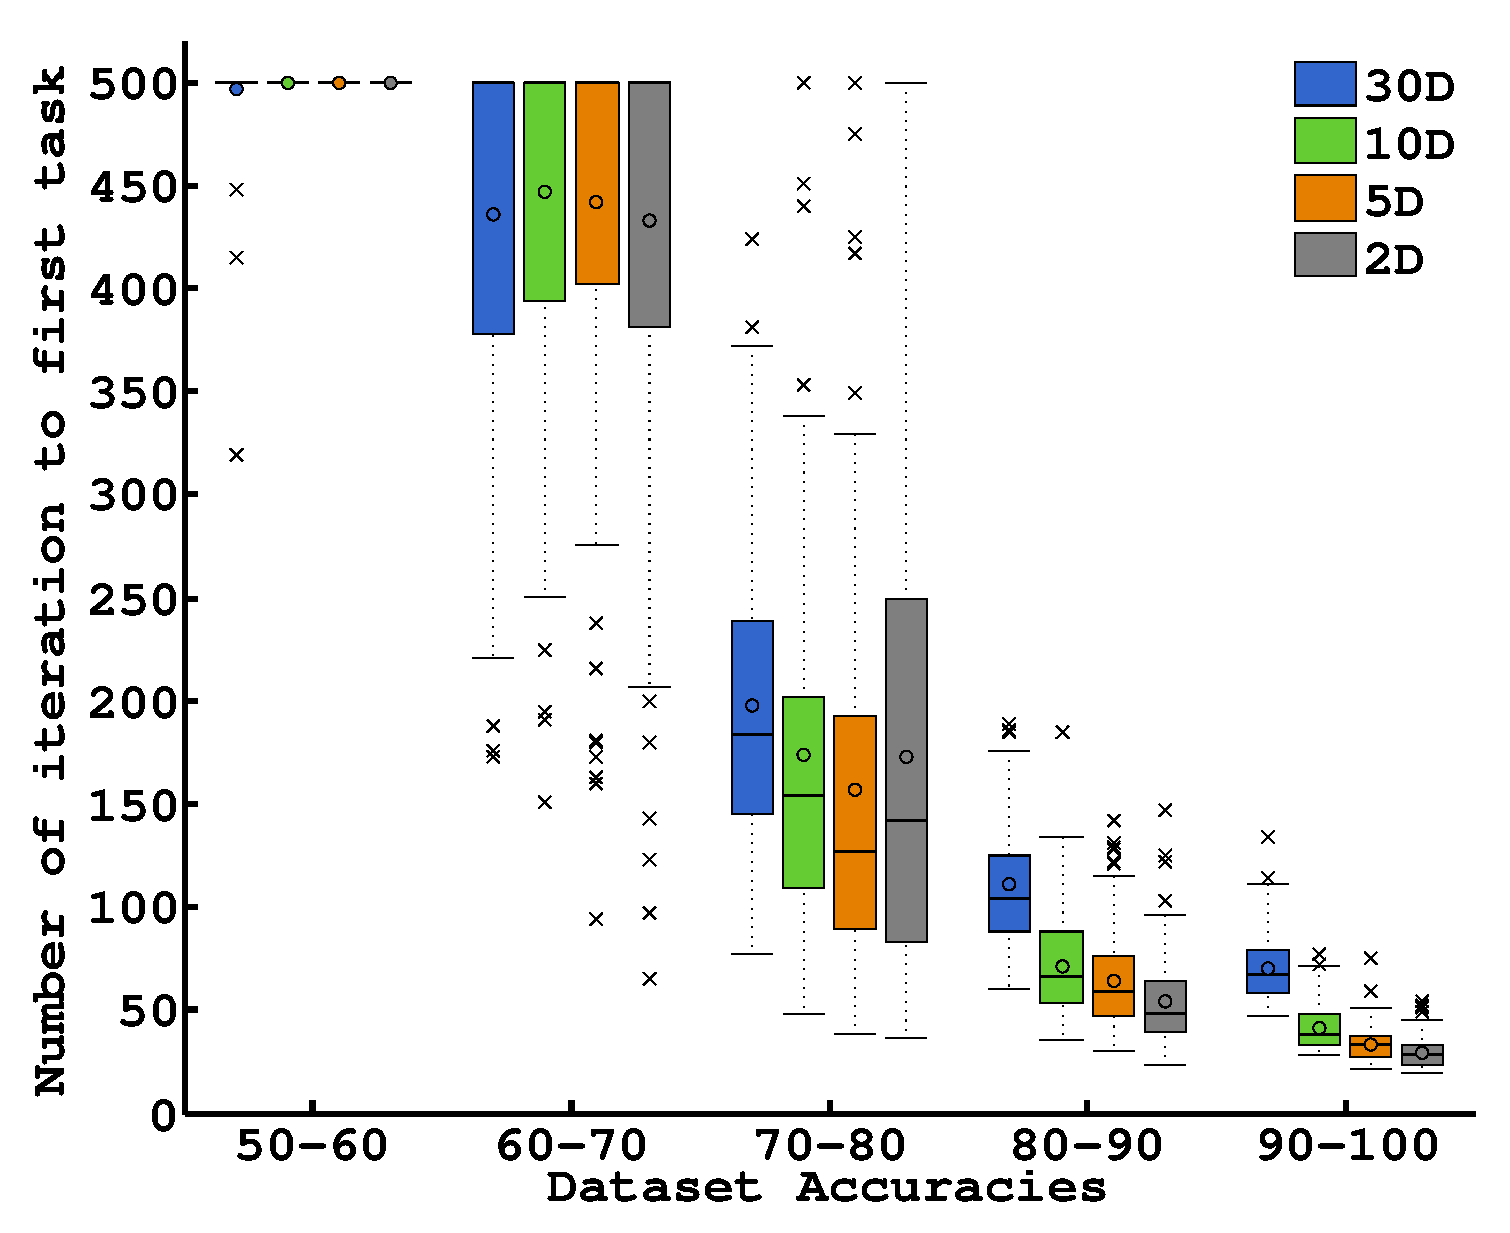
\includegraphics[width=\plotsize\columnwidth]{\imgpath/plot_artificial_firstconf.eps}
%       \caption{Under 70 percent accuracy, the confidence threshold cannot be reached in 500 steps. The dataset qualities, more than their dimensionality, impact the learning time.}
%       \label{fig:firstArtificial}
% \end{minipage}  
% \begin{minipage}[t]{.65\columnwidth}
%   \centering
%         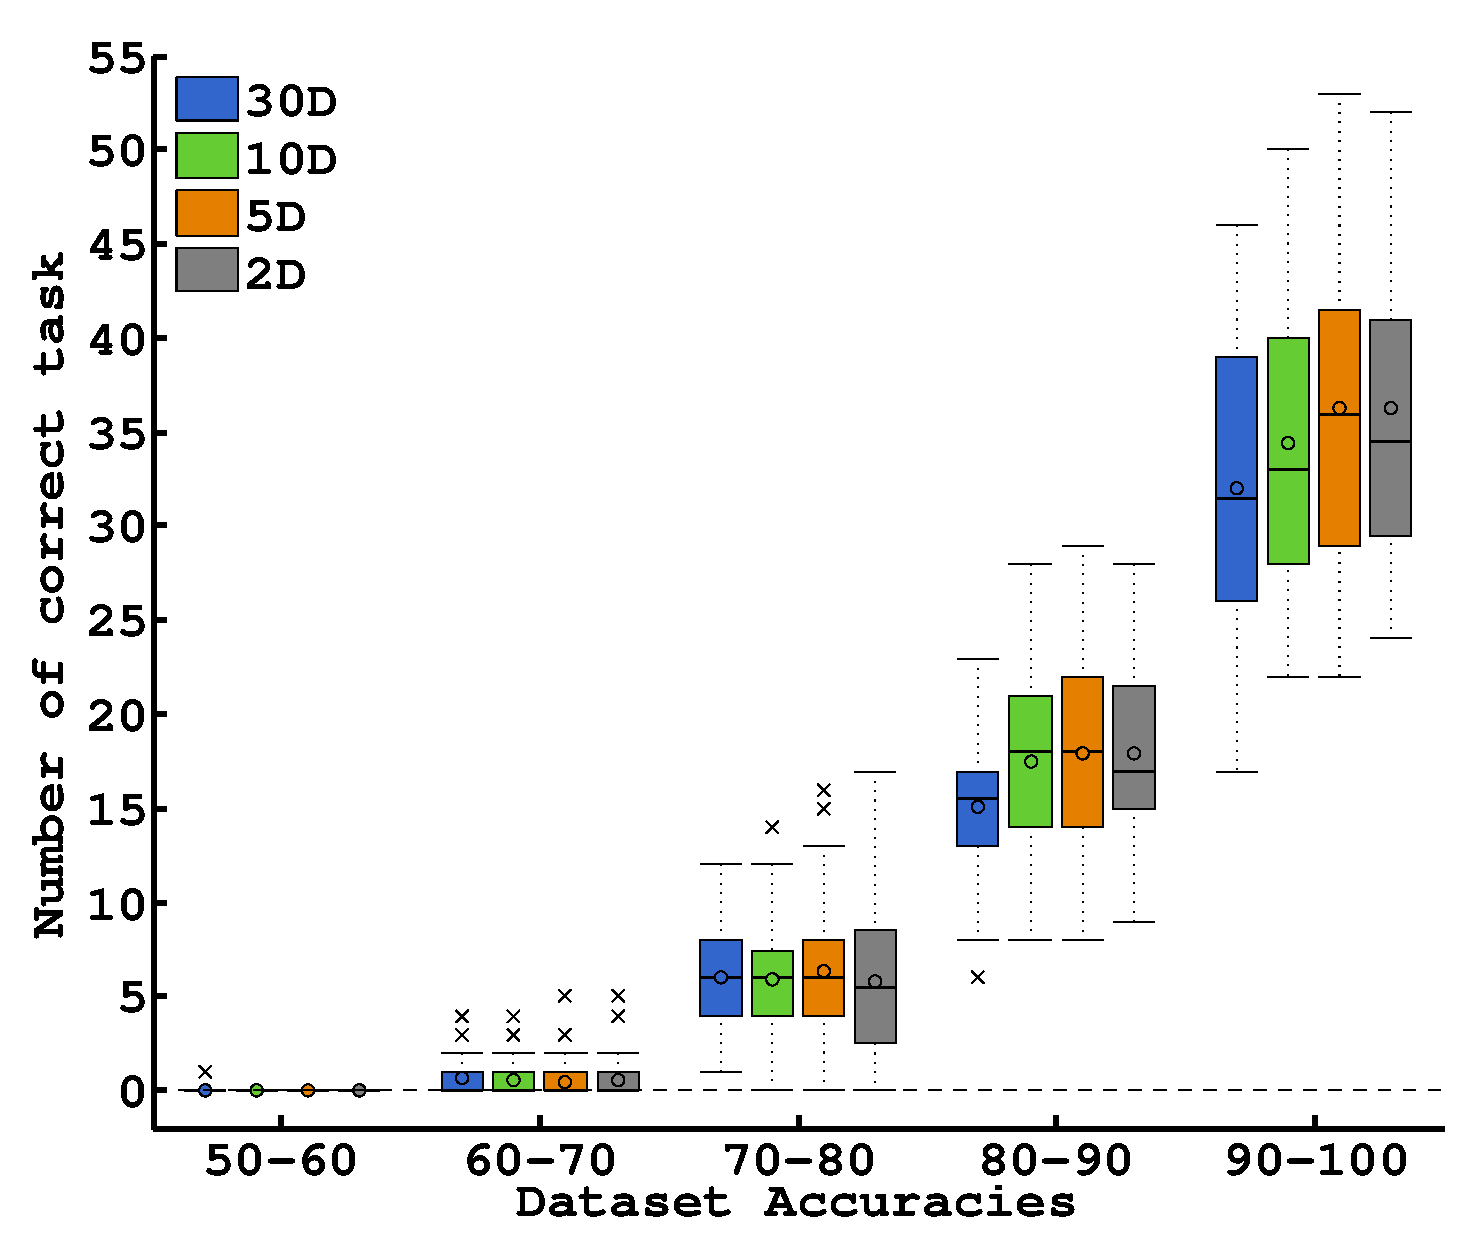
\includegraphics[width=\plotsize\columnwidth]{\imgpath/plot_artificial_nCorrect.eps}
%       \caption{Quality of dataset impacts the number of task identified in 500 steps, more evidence should be collected to reach the confidence threshold.}
%       \label{fig:nCorrectArtificial}
% \end{minipage}
% \end{figure*} 

% \begin{figure}[t]
% \centering
% 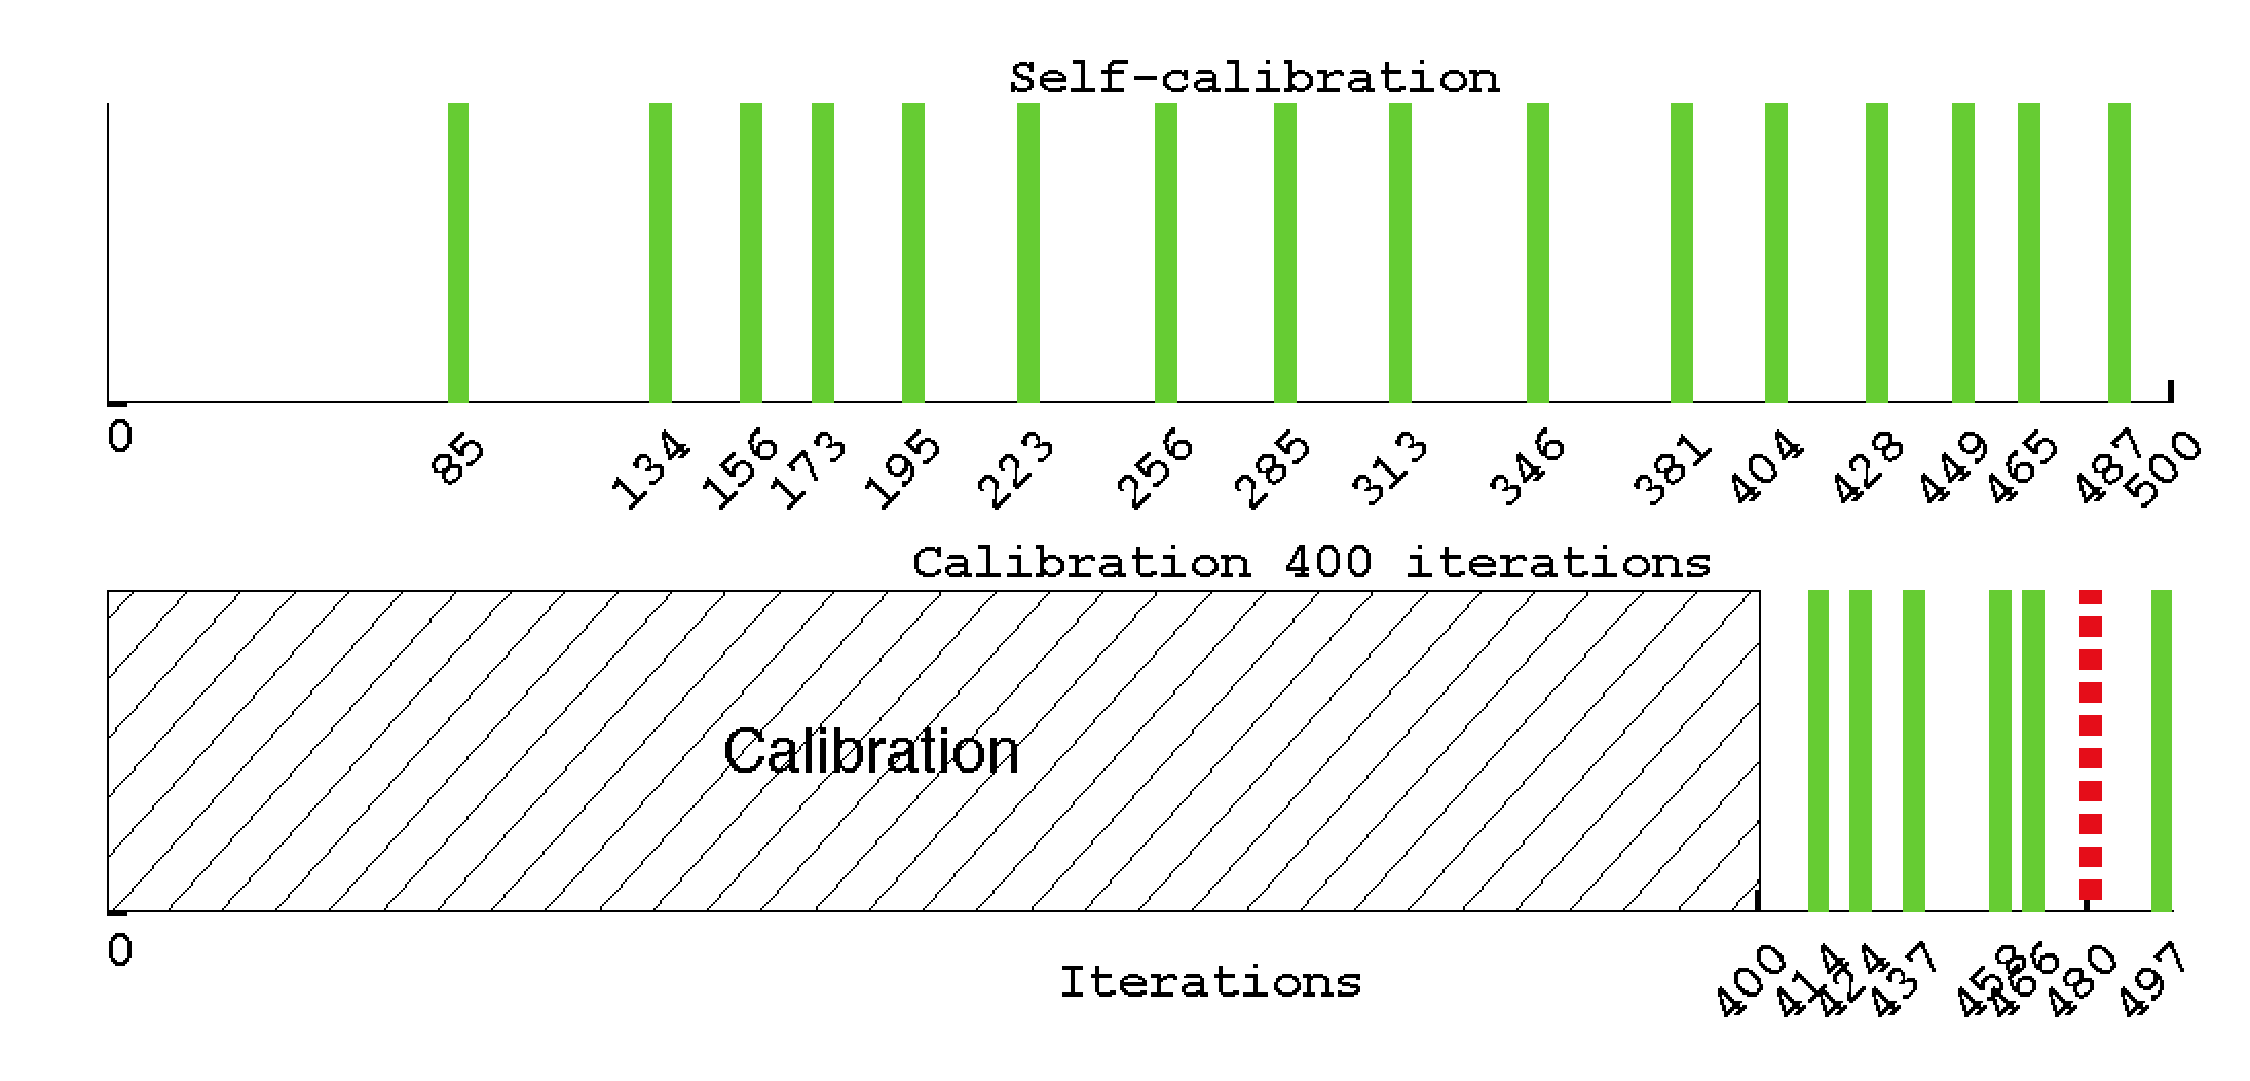
\includegraphics[width=\plotsize\columnwidth]{\imgpath/plot_the_aaai_sequence.eps}
% \caption{The proposed self-calibration method allow to reach a first task faster, with performance increasing with time. One run from EEG dataset of 83 percent accuracy, self-calibration versus 400 steps calibration.}
% \end{figure} 
